\documentclass[10pt]{beamer}

%\usetheme{Montpellier}
\usetheme{Madrid}

\usecolortheme{beaver}
\usepackage{appendixnumberbeamer}
\usepackage[utf8]{inputenc}
\usepackage[spanish]{babel}
\usepackage{booktabs}
\usepackage[scale=2]{ccicons}
\usepackage{pgfplots}
\usepackage{framed}
\usepgfplotslibrary{dateplot}
\usepackage{xspace}
\usepackage{csquotes}
\usepackage{graphicx}
\usepackage{verbatim}
\usepackage{listings}

%\usefonttheme{professionalfonts}
%\usefonttheme{serif} % default family is serif
%\usepackage{fontspec}
%\setmainfont{Liberation Serif}
\newcommand\IncrFont{\fontsize{20}{20}\selectfont}
\newcommand{\themename}{\textbf{\textsc{metropolis}}\xspace}
\graphicspath{ {../images/} }
\newcommand{\norm}[1]{\left\lVert#1\right\rVert}


\title{Detalles - QyA}
%\subtitle{Trabajo Final de Grado, Licenciatura en Ciencias de la Computación}

\date{Diciembre de 2018}

\author{Juan M. Scavuzzo}
\institute{Facultad de Matemática, Astronomía, Física y Computación \\ Universidad Nacional de Córdoba}
\titlegraphic{
\includegraphics[width=\textwidth,height=.3\textheight]{titulo_mosq}}
\begin{document}

\maketitle



\begin{frame}{}
  \IncrFont
  \begin{center}
    \textit{\textbf{Variables Ambientales utilizadas para NED}}
  \end{center}
\end{frame}

\begin{frame}
  \begin{itemize}
    \item MODIS
      \begin{itemize}
        \item Valores medios mensuales de NDVI
      \end{itemize}
    \item Wordclim
      \begin{itemize}
        \item BIO1 = Annual Mean Temperature
        \item BIO2 = Mean Diurnal Range (Mean of monthly (max temp - min temp))
        \item BIO3 = Isothermality (BIO2/BIO7) (* 100)
        \item BIO4 = Temperature Seasonality (standard deviation *100)
        \item BIO5 = Max Temperature of Warmest Month
        \item BIO6 = Min Temperature of Coldest Month
        \item BIO7 = Temperature Annual Range (BIO5-BIO6)
        \item BIO8 = Mean Temperature of Wettest Quarter
        \item BIO9 = Mean Temperature of Driest Quarter
        \item BIO10 = Mean Temperature of Warmest Quarter
        \item BIO11 = Mean Temperature of Coldest Quarter
        \item BIO12 = Annual Precipitation
        \item BIO13 = Precipitation of Wettest Month
        \item BIO14 = Precipitation of Driest Month
        \item BIO15 = Precipitation Seasonality (Coefficient of Variation)
        \item BIO16 = Precipitation of Wettest Quarter
        \item BIO17 = Precipitation of Driest Quarter
        \item BIO18 = Precipitation of Warmest Quarter
        \item BIO19 = Precipitation of Coldest Quarter
      \end{itemize}
  \end{itemize}
\end{frame}



\begin{frame}{}
  \IncrFont
  \begin{center}
    \textit{\textbf{Algoritmos utilizados}}
  \end{center}
\end{frame}



\begin{frame}{Algoritmos utilizados: KNNR}
  \begin{itemize}
    \item Utiliza los $K$ puntos conocidos más cercanos para predecir el nuevo
    \item En regresión, el valor predicho suele ser el promedio del valor de los $K$ vecinos más cercanos
  \end{itemize}
\end{frame}


\begin{frame}{Algoritmos utilizados: DTR}
  \begin{itemize}
    \item Método no-paramétrico de aprendizaje supervisado
    \item Usado tanto para regresión como clasificación
    \item Estructura Arbórea: nodos de decisión, nodos hojas
    \item Proceso iterativo de división de los datos
  \end{itemize}
  \pause
  Supongamos que los datos del nodo $m$ son representados por $Q$
  \begin{itemize}
    \item Para cada candidato se divide en $Q_{izq}(\theta)$ y $Q_{der}(\theta)$
    donde
      \begin{itemize}
        \item $\theta\ =\ (j, t_{m})$,
          $j$ es una característica y $t_{m}$ es el humbral
        \item $Q_{izq}(\theta) = (x, y) | x_{j} \leq t_m$ \\
        $Q_{der}(\theta) = Q - Q_{izq}(\theta)$
      \end{itemize}
  \end{itemize}

\end{frame}


\begin{frame}{Algoritmos utilizados: DTR}
  \begin{itemize}
    \item Supongamos que hay $N(m)$ observaciones
    \item En cada paso, se busca minimizar la función $m$
      \begin{center}
        $G(Q, \theta) = \frac{n_{izq}}{N_{m}} \ H(Q_{izq}(\theta)) + \frac{n_{der}}{N_{m}} \ H(Q_{der}(\theta))$
      \end{center}
      donde $H()$ es la función de impureza de $m$
      \item En regresiones, la funcion de impureza suele ser el MSE o el MAE
      \item Luego, se seleccionan los parámetros tal que
      \begin{center}
        $\theta^{*} = argmin_{\theta} \ G(Q, \theta)$
      \end{center}
  \end{itemize}
\end{frame}


\begin{frame}{Algoritmos utilizados: SVR}
  \begin{itemize}
    \item Construye un hiperplano o un conjunto de hiperplanos en un espacio de muy alta dimensionalidad
  \end{itemize}
  \begin{center}
    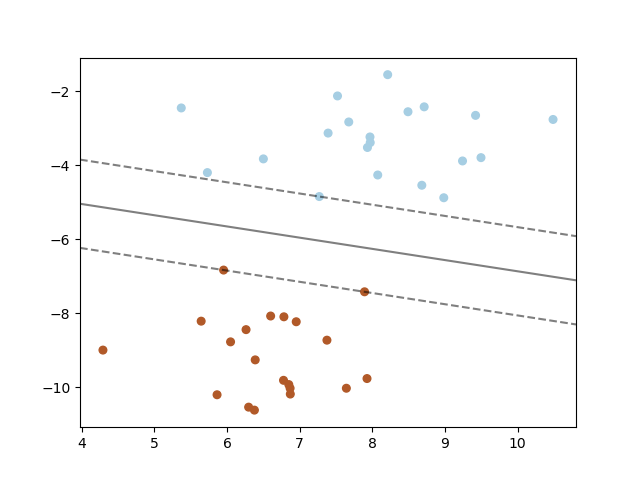
\includegraphics[width=0.7\textwidth]{svm_hiperplane}
  \end{center}
\end{frame}


\begin{frame}{Algoritmos utilizados: SVR}
  \begin{itemize}
    \item Busca aproximar la función desconocida $F(\vec{X}) = \vec{Y}$
    \item Los $\vec{X}$ son utilizados para definir los hiperplanos que separa las soluciones
    \item En el caso de regresión, se utilizan los hiperplanos para ajustar la curva
    \item Se tiene una tolerancia de $\epsilon$ para cada punto
  \end{itemize}
\end{frame}



\begin{frame}{Algoritmos utilizados: MLP}
  \begin{itemize}
    \item Es un tipo de ANN \textit{feedforward}
    \item Utiliza \textit{backpropagation}
    \item Tiene, al menos tres capas: capa de entrada, capa oculta, capa de salida.
  \end{itemize}
  \begin{center}
    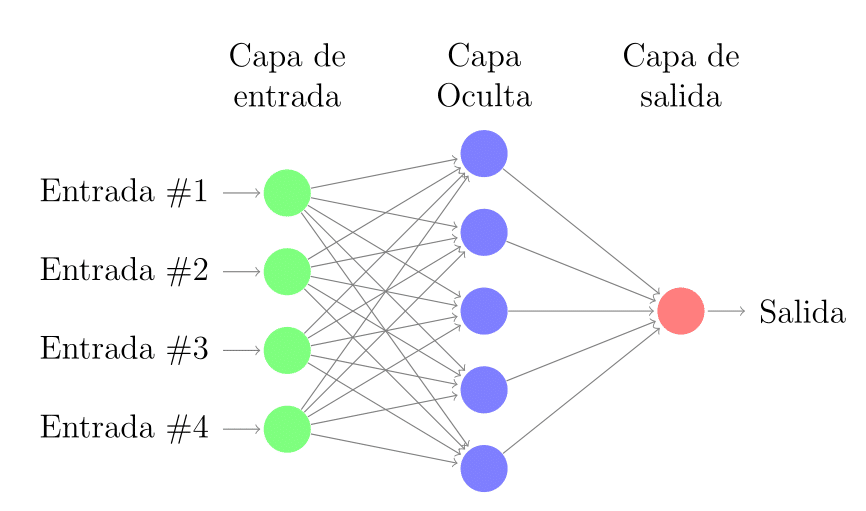
\includegraphics[width=0.7\textwidth]{ejemplo_mlp}%
  \end{center}
\end{frame}




\begin{frame}{Algoritmos utilizados: MLP}
  Para una MLP de una capa oculta con una sola neurona
  \begin{itemize}
    \item Dados datos de entrenamiento $(x_{1}, y_{1}), \dots, (x_{n}, y_{n})$
    donde $x_{i} \in \mathbb{R}^{m}$
    \item Aprende la función
      \begin{center}
        $f(x) = W_{2}g(W_{1}^{T} x + b_{1}) + b_{2}$
      \end{center}
      donde
        \begin{itemize}
          \item $W_{1} \in \mathbb{R}^{m}$ y $W_{2}, b_{1}, b_{2} \in \mathbb{R}$ son parámetros del modelo
          \item $W_{1}, W_{2}$ representan los pesos de la capa de entrada y la capa oculta
          \item $b_{1}, b_{2}$ representan el sesgo agregado a la capa oculta y la capa de salida
          \item $g(): \mathbb{R} \rightarrow \mathbb{R}$ es la función de activación
        \end{itemize}

  \end{itemize}
\end{frame}

\begin{frame}{Algoritmos utilizados: MLP}
  \begin{itemize}
      \item En problemas de regresión, la salida del algoritmo es $f(x)$ por lo que $g()$ es la identidad
      \item Utiliza como función de pérdida el \textit{Error Cuadrático}
        \begin{center}
          $Loss(\hat{y}, y, W) = \frac{1}{2} \norm{\hat{y} - y}^{2}_{2} + \frac{\alpha}{2} \norm{W}^{2}_{2}$
        \end{center}
      \item Luego
      \begin{center}
        $W^{i + 1} = W^{i} - \epsilon \nabla Loss^{i}_{W}$
      \end{center}
    \end{itemize}
\end{frame}



\end{document}
